\PassOptionsToPackage{dvipsnames}{xcolor}
\documentclass{article}
\usepackage{graphicx}
\usepackage[dvipsnames]{xcolor}
\usepackage{amsmath,amssymb,enumerate,graphicx,pgf,tikz,fancyhdr}
\usepackage{hyperref}
\usepackage{geometry}
\usepackage{tabvar}
\usepackage{fontspec}
\usepackage{dot2texi}
\usepackage{minted}
\usetikzlibrary{backgrounds}
\usetikzlibrary{arrows.meta}
\usetikzlibrary{shapes.geometric}

\title{\centering Majeure Informatique: 
Jeu d'échecs}

\author{BOYER Timothé, MOURET Basile, HACINI Malik}
\date{26 Septembre 2023}
\renewcommand{\contentsname}{Table des Matières}

\renewcommand{\theFancyVerbLine}{
    \sffamily\textcolor[rgb]{0.5,0.5,0.5}{\scriptsize\arabic{FancyVerbLine}}}
    
    
\begin{document}
    
    
\csundef{listing}\csundef{endlisting}
\csundef{listing*}\csundef{endlisting*}

\maketitle
\tableofcontents{}

\section{Introduction}
L’objectif de ce projet est de programmer (et tester) un jeu
d’échecs qui permet à deux joueurs de s’affronter, 
chaque joueur peut être soit un humain, soit l’ordinateur via une IA
 (intelligence artificielle) . Le jeu se jouera dans un terminal, 
 et si les deux joueurs sont humains, ils utiliseront le même clavier.
 \section{Collaboration}
 
Pour ce projet, nous avons mis en place un \href{https://github.com/Zertag/Projet-POO}{\textcolor{blue}{dépôt GitHub}}, qui a nous a permis
de chacun travailler sur sa propre version du projet avec VS Code (dépôt cloné localement) et 
ensuite de plus facilement mettre a jour le projet pour tout le monde.
Cependant, ce projet était pour nous tous notre premier contact avec Git et Github, donc
nous n'avons certainement pas utilisé l'outil à son plein potentiel. Nous avons notamment
plusieurs fois du traiter manuellement des conflits de fusion, lorsque la répartition
des tâches n'était pas assez bien réalisée.
Dans l'ensemble, notre collaboration fut tout de même fluide et efficace.
\section{Conception}
\subsection{Règles traitées}
Le jeu d'échecs comporte plusieurs règles spéciales (Promotion, Roque, prise en passant...)
Cependant, bon nombres d'entre elles sont plutôt fastidieuses à mettre en place,
et ne sont pas forcément essentielles au déroulement du jeu.
Nous avons donc seulement implémenté la Promotion.

La gestion de la nullité de la partie mérite aussi de s'y attarder.
Nous avons longtemps hésité sur la méthode à mettre en place pour gérer la nullité de la partie.

\subsection{Architecture}
Ce projet a été réalisé en utilisant les outils de la programmation orientée objet (POO).
Les différentes composantes d'un jeu d'échecs (joueurs, pieces) sont donc 
représentées par des classes.
\subsubsection{Diagramme de classe UML}
a mettre


Il y eu 2 grandes phases de développement du projet : La conception du jeu entre humains
et la mise en place de l'IA. Chaque phase à donné lieu à plusieurs algorithmes principaux que nous allons détailler.
Evidemment, nous avons rencontré de nombreuses difficultés, que nous détaillerons, durant chaque étape de la conception.

\subsection{Conception du Jeu d'échecs}
Nous avons commencé par créer en parallèle les 3 classes constituantes du jeu:
Piece, EtatJeu et Joueurs. Ces classes sont toutes associées (CF 2.2.1), donc
nous ne les avons pas réellement rédigés indépendamment.
\subsubsection{Classe Piece}
La classe Piece et ses sous-classes sont les lieux ou les règles du jeu sont définies.
On représente chaque type de pièce par une sous-classe de la classe Piece.
Chacune de ses pieces possède sa propre méthode (overwrite) coups-possibles, qui encode les règles du jeu
qui lui sont relatives. Ces méthodes nécéssitent évidemment d'avoir accès a l'état du jeu.
Enfin, la classe Piece possède une méthode coups-légaux (donc identique pour tout les types de pièces)
qui trie une liste de coups possibles en enlevant ceux qui mettent en échec le roi.
Ces méthodes nécéssitent évidemment d'avoir accès a l'état du jeu, que nous avons donc défini par la suite.
\paragraph{Difficultés}
Nous avons débuté  l'implémentation de la classe Piece très tôt dans la conception. Cependant, la méthode 
coups-légaux était très compliquée à mettre en place : nous n'avions pas encore
de moyen de vérifier si un roi était un échec. Nous avons donc du mettre en pause
la conception de la classe Piece. A ce stade là, voici son corps : 


\begin{minted}[mathescape,
    linenos,
    numbersep=5pt,
    gobble=2,
    frame=lines,
    framesep=2mm]{python}

    #PLACEHOLDER
\end{minted}
\subsubsection{Classe EtatJeu}
\paragraph{Plateau: Création, Affichage et Sauvegarde}
Nous avons d'abord mis en place le plateau, ainsi que l'affichage de celui-ci.
\begin{minted}[mathescape,
    linenos,
    numbersep=5pt,
    gobble=2,
    frame=lines,
    framesep=2mm]{python}

    #PLACEHOLDER
\end{minted}

Plusieurs choix importants ont été réalisés pour la mise en place du plateau:
Nous le représentons via un dictionnaire, contenant des coordonnées (tuple) en clé
et des pièces (objets de la classe Piece) en valeur. Cette réprésentation
possède plusieurs avantages: Il est facile d'accéder au symbole UTF-8 des pièces
pour l'affichage, à la couleur d'une pièce, ou même à ses coups possibles.

Aussi, un objet EtatJeu possède une liste de deux listes de pièces, les blanches et les noires.
L'accès au pièces noires ou blanches est réalisé en accédant au bone indice de la liste pieces via
le trait.

Pour la sauvegarde, nous avons commencé par en implémenter une, puis nous l'avons modifié par la suite.
Notre première méthode de sauvegarde était basée sur le dictionnaire des pièces.
On sauvegardait, dans un fichier texte, les éléments nécéssaires à la construction des objets Piece (type,couleur,position).

Cependant, par la suite, cette méthode nous a gênée. Pour tester le programme, nous avions besoin de pouvoir
rapidement générer des plateaux avec une situation exacte. Cependant, notre sauvegarde n'étant pas pratique à manipuler,
nous devions constamment jouer, sur le programme, les coups exacts pour arriver à la situation souhaitée. Cela était
fastidieux, et très inefficace. 
Nous avons donc opté pour une sauvegarde adoptant la \href{https://fr.wikipedia.org/wiki/Notation_Forsyth-Edwards}{\textcolor{blue}{notation Forsyth-Edwards}} (FEN).
Cette notation est utilisée dans la plupart des chess engine actuels. Elle nous a ensuite permis de créer les sauvegardes
de tests souhaitées grâce à un outil de \href{https://lichess.org/fr}{\textcolor{blue}{Lichess}}.

Voici l'implémentation finale de la sauvegarde :
\begin{minted}[mathescape,
    linenos,
    numbersep=5pt,
    gobble=2,
    frame=lines,
    framesep=2mm]{python}

    #PLACEHOLDER
\end{minted}

\paragraph{Vérification de l'état du jeu}
Nous devions donc maintenant ajouter les fonctions relatives à la vérification de l'état du jeu
: échec, échec et mat, égalité. 

Les fonctions échec et échec et mat sont assez explicites :
\begin{minted}[mathescape,
    linenos,
    numbersep=5pt,
    gobble=2,
    frame=lines,
    framesep=2mm]{python}

    #PLACEHOLDER
\end{minted}

Pour l'égalité, c'est plus compliqué.
Aux échécs, il existe une multitude de manières de rendre en partie nulle. Cependant, beaucoup d'entres elles sont 
très complexes à mettre en place. Un exemple sera le plus parlant : 

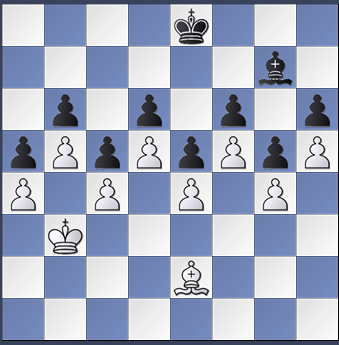
\includegraphics{exempledraw}

Aux yeux d'un joueur d'échec, cette partie est très clairement une nulle.
Cependant, il est très complexe pour un algorithme de le reconnaître.
Nous ne pouvons donc pas mettre en place toutes les possibilités différentes.

Notre gestion de la nulle est donc assez basique, nous ne vérifions que 2 cas particuliers.

Premièrement, nous vérifions la règle du pat : un des joueurs n'a aucun coup possible, mais il n'est pas en échec en mat.
Ensuite, on annonce nulle si un des deux rois à bougé plus de 30 fois d'affilé.
Enfin, à chaque tour, les joueurs peuvent conjointement décider de terminer sur un nul.
 
Voici l'implémentation des deux cas particuliers: 
\begin{minted}[mathescape,
    linenos,
    numbersep=5pt,
    gobble=2,
    frame=lines,
    framesep=2mm]{python}

    #PLACEHOLDER
\end{minted}


\subsubsection{Finalisation de la classe Piece}
Une fois l'EtatJeu mis en place, nous pouvons écrire la méthode coups légaux.

\begin{minted}[mathescape,
    linenos,
    numbersep=5pt,
    gobble=2,
    frame=lines,
    framesep=2mm]{python}

    #PLACEHOLDER
\end{minted}

\subsubsection{Classe Joueurs : Humain}
A ce stade, le noyau du jeu d'échecs est terminé. Pour le rendre jouable,
nous devons implémenter la classe Joueurs.
C'est la classe Joueurs qui sera, durant la partie, l'interface entre le programme main et les
classes Piece et EtatJeu, via la méthode jouer-coup.\\ En prévision de l'implémentation de l'IA,
on implémente une sous classe Humain, qui a sa propre méthode jouer-coup, car celle de l'IA sera différente.
Pour la classe Humain, la méthode jouer-coup doit interagir avec l'utilisateur. \\
On doit notamment effectuer la conversion des coordonnées du plateau en notation algébrique.


\begin{minted}[mathescape,
    linenos,
    numbersep=5pt,
    gobble=2,
    frame=lines,
    framesep=2mm]{python}

    #PLACEHOLDER
\end{minted}


\subsection{Le Programme main}
Au final, le jeu doit se joueur depuis un simple script main, qui utilise nos classes
définies dans des fichiers annexes.
Nous avons décidé d'implémenter ce programme avant de concevoir l'IA, 
afin de faciliter les tests.
On définit alors une fonction partie, qui créee (à partir des choix de l'utilisateur) et fait jouer une partie à l'utilisateur.
Cette fonction doit notamment gérer le vote de la nulle.
On place ensuite cette fonction dans une boucle, en demandant à l'utilisateur si il veut rejouer
à chaque fin de partie.
\begin{minted}[mathescape,
    linenos,
    numbersep=5pt,
    gobble=2,
    frame=lines,
    framesep=2mm]{python}

    #PLACEHOLDER
\end{minted}
\subsection{Conception de l'IA}
Notre IA sera basée sur l'algorithme minimax et l'élagage alphabeta.
Pour implémenter l'IA, nous nous y sommes repris plusieurs fois.
Nous avons essuyé plusieurs difficultés : valeur erronée, problèmes de récursivité, coups absurdes de l'IA etc.
Notre première difficulté fut rencontré lors de l'élaboration de la fonction de calcul de valeur du jeu.

\subsubsection{Calcul de la valeur}

Pour évaluer la partie, nous avons longtemps cherché la méthode correcte. 
La base de notre méthode heuristique
est la fonction d'évaluation de Claude Shannon. C'est une fonction symétrique : si l'avantage est aux blancs,
la valeur sera positive, si l'avantage est aux noirs, elle sera négative.
Le critère principal est le barème général de la valeur des pièces aux échecs : \\

\begin{center}
\begin{tabular}{ |p{1cm}||p{1cm}|p{1cm}|p{1cm}|p{1cm}|p{1cm}|  }
    \hline
    \multicolumn{6}{|c|}{Valeurs des pièces} \\
    \hline 
    Roi&Pion&Cavalier&Fou&Tour&Dame \\ 
    \hline 
1000&1&3&3&5&9 \\
\hline
\end{tabular} 
\end{center}

Cependant, cette base n'était pas suffisante pour obtenir une valeur reflétant correctement le jeu d'échecs.
Nous avons donc pris plusieurs critères en compte :
\begin{itemize}
    \item Si les pièces sont au centre ou au sous-centre du plateau (augmentation de la valeur)
    \item Le nombre de cases accessibles au prochian tour (appelées cases controlées, augmentation de la valeur)
    \item L'alignement des pions (baisse de la valeur)
\end{itemize}

Evidemment, cette liste n'est absolument pas exhaustive et est loin de représenter parfaitement 
toute la complexité du jeu d'échecs. De plus, le poids que nous avons attribué à chaque critère se base
sur des méthodes déjà existantes, mais une part d'arbitraire rentre en compte. 
En revanche, il n'y aurait que peu d'intêret à avoir une fonction valeur extrêmemnt élaborée.
En effet, notre IA ne pourra que se contenter d'une profondeur de 3 au maximum (à partir de 4, c'est trop long en pratique),
et les effets d'une valeur plus précise ne se feront donc pas énormément ressentir pour la majorité de la partie.
Vers la fin de la partie, l'impact est plus grand.


Nous avons testé plusieurs versions, mais voici la version finale du calcul de la valeur:  
\begin{minted}[mathescape,
    linenos,
    numbersep=5pt,
    gobble=2,
    frame=lines,
    framesep=2mm]{python}

    #PLACEHOLDER
\end{minted}

\subsubsection{Minimax}
Pour implémenter Minimax, nous nous sommes basés sur l'algorithme du cours.
Il faut cependant pouvoir passer la profondeur comme un paramètre.
Nous ne rédigons pas la fonction dans la classe Joueurs, du à sa nature récursive.
C'est la méthode jouer coup d'un joueur IA qui y fera appel.
L'algorithme minimax impose de simuler des coups.
En première approche, nous avons implémenté la méthode suivante : \\
\begin{itemize}
    \item On copie l'état de jeu avec un deepcopy 
    \item On joue un coup sur ce nouvel état, et on calcule la valeur
    \item On renvoie la valeur
\end{itemize}

Cependant, nous nous sommes rendus compte de l'inefficacité de la méthode en la testant.
La création d'un nouvel objet EtatJeu à chaque itération de la fonction était très longue,
et remplissait la mémoire. Avec cette méthode (sans élagage alpha\-beta), une IA de profondeur 3
mettait plus de 1 min a donner un coup. \\

Nous avons alors modifié notre approche.
\begin{itemize}
    \item On sauvegarde les informations qui seront modifiées (positions de la pièce déplacée, pièce mangée, odomètre du roi)
    \item On simule directement le coup sur l'état de jeu.
    \item On calcule la valeur.
    \item On restaure le jeu à son état initial.
\end{itemize}
Avec cette nouvelle approche, le temps d'obtention d'un coup d'une IA de profondeur 3 passe à 30 secondes.

Voici l'implémentation finale de la fonction minimax :

\begin{minted}[mathescape,
    linenos,
    numbersep=5pt,
    gobble=2,
    frame=lines,
    framesep=2mm]{python}

    #PLACEHOLDER
\end{minted}


\subsubsection{Elagage Alpha-Beta}
L'élagage alpha-beta n'améliore pas la qualité des coups de l'IA, mais réduit significativement la durée des coups.
Nous nous sommes basés sur l'algorithme vu en cours.
En voici l'implémentation :
\begin{minted}[mathescape,
    linenos,
    numbersep=5pt,
    gobble=2,
    frame=lines,
    framesep=2mm]{python}

    #PLACEHOLDER
\end{minted}
Grâce à cette amélioration, une IA de profondeur 3 joue maintenant en 15 secondes en moyenne. (Nous avons établi cette
valeur grâce à un test, détaillé dans la section prévue à cet effet.)
\subsubsection{Méthode Jouer\_Coup pour l'IA}
Malgré sa présence à cet endroit dans le rapport, nous avons écrit la méthode jouer\_coup assez tôt dans la conception de l'IA.
Cela nous permettait de tester eficacement nos algorithmes alpha\_beta et minimax.
Sa version finale fut cependant rédigée à la fin du processus.
Cette méthode met en place la version complète d'un minimax avec élagage Alpha\-Beta, c'est elle qui
trouve et choisit le meilleur coup possible à une certaine profondeur.

La voici:
\begin{minted}[mathescape,
    linenos,
    numbersep=5pt,
    gobble=2,
    frame=lines,
    framesep=2mm]{python}

    #PLACEHOLDER
\end{minted}

\section{Tests}
Dans cette partie du compte rendu, nous nous intéresserons aux tests réalisés sur les différentes parties de notre programme.

\subsection{Tests de conception du jeu d'échecs}
Nous avons réalisé des tests sur les différents programmes qui permettent au jeu d'échecs de fonctionner.

Pour tester le bon fonctionnement du jeu, nous avons utilisé la fonctionnalité nous permettant d'importer des sauvegardes car ainsi, on peut tester des situations précises et voir si tout fonctionne comme prévu.
\\
On crée donc une fonction dont le but est de créer des parties à partir du nom du fichier de test. Cela nous permet de ranger les tests dans différents dossiers dédiés à chaque test.

\subsubsection{Tests de la classe pièce}
Pour tester les pièces, nous avons d'abord testé la méthode coups\_possibles pour chacune des pièces existantes. Pour cela, nous avons d'abord créé une situation avec la pièce que l'on veut tester. On note à la main toutes les cases accessibles par cette pièce et on vérifie si la méthode coups\_possibles de cette pièce renvoie la même liste de coups.

\begin{minted}[mathescape,
    linenos,
    numbersep=5pt,
    gobble=2,
    frame=lines,
    framesep=2mm]{python}
    # Déplacement des pièces
    def test_deplacement_pion():
        partie=init_partie_test("test_deplacement_pion")
        partie.pieces[1][1].premier_coup=False
        assert partie.pieces[1][0].coups_possibles(partie)==[(3, 4), (4, 4)]
        assert partie.pieces[1][1].coups_possibles(partie)==[]
        assert partie.pieces[1][2].coups_possibles(partie)==[(1, 2), (1, 3)]
    
    def test_deplacement_fou():
        partie=init_partie_test("test_deplacement_fou")
        assert partie.pieces[1][0].coups_possibles(partie)==[(5,5),(6,6),(7,7),(5,3),(3,3),(2,2),
        (1,1),(3,5),(2,6),(1,7)]
                
    def test_deplacement_tour():
        partie=init_partie_test("test_deplacement_tour")
        assert partie.pieces[0][1].coups_possibles(partie)==[(5, 4), (6, 4), (7, 4), (4, 5), 
        (3, 4), (2, 4), (1, 4), (4, 3), (4, 2), (4, 1)]
    
    
    def test_deplacement_reine():
        partie=init_partie_test("test_deplacement_reine")
        assert partie.pieces[0][0].coups_possibles(partie)==[(5, 5), (6, 6), (5, 3), (3, 3), 
        (2, 2), (1, 1), (0, 0), (3, 5), (2, 6), (1, 7), 
        (5, 4), (6, 4), (7, 4), (4, 5), (4, 6), (4, 7), (3, 4), 
        (2, 4), (4, 3)]
    
    def test_deplacement_cavalier():   
        partie=init_partie_test("test_deplacement_cavalier")
        assert partie.pieces[1][1].coups_possibles(partie)==[(5, 5), (3, 5), (2, 4), (2, 2), 
        (3, 1), (5, 1), (6, 2)]
\end{minted}


Il faut ensuite vérifier si il est bien impossible de déplacer une pièce en mettant le roi en échec. 
Cette fonctionnalité correspond à la méthode coups\_legaux de la classe Pièce. 
Pour vérifier si ça marche, on fait donc un plateau avec une pièce qui est clouée (si elle bouge, le roi est en échec) et on vérifie qu'elle n'a pas de coups légaux.

\begin{minted}[mathescape,
    linenos,
    numbersep=5pt,
    gobble=2,
    frame=lines,
    framesep=2mm]{python}
    def test_coups_legaux():
        partie=init_partie_test("test_coups_legaux")
        assert partie.pieces[1][0].coups_possibles(partie)==[(5, 3), (3, 3), (2, 2), (2, 0), 
        (6, 0), (6, 2)]
        assert partie.pieces[1][0].coups_legaux(partie)==[]
\end{minted}

\subsubsection{Tests de l'ÉtatJeu}
\paragraph{Tests des échecs}

Nous avons fait différents tests pour voir si les méthodes echec et echec\_et\_mat fonctionnent correctement. Pour cela, on crée 3 situations :
\begin{itemize}
    \item Une avec le joueur qui doit jouer en échec
    \item Une sans échec et donc sans mat
    \item Une autre où le joueur qui doit jouer est en échec et mat
\end{itemize}

\begin{minted}[mathescape,
    linenos,
    numbersep=5pt,
    gobble=2,
    frame=lines,
    framesep=2mm]{python}
    def test_pat():
        # 1ère situation de nulle, il n'y a pas d'échec et mat et aucun coup n'est possible
        partie=init_partie_test("pat_1")
        assert partie.pat()
        # 2ème situation de nulle, seul les rois bougent
        partie=init_partie_test("pat_2")
        partie.pieces[1][0].odometre=40
        assert partie.pat()
        
    def test_echec():
        partie=init_partie_test("avec_echec")
        assert partie.echec()
        partie=init_partie_test("sans_echec")
        assert not partie.echec()
    
    def test_mat():
        partie=init_partie_test("avec_mat")
        assert partie.echec_et_mat()
        partie=init_partie_test("sans_mat")
        assert not partie.echec_et_mat()
\end{minted}

\subsection{Tests relatifs à l'IA}
\subsubsection{Tests de la valeur} 
Pour tester le calcul de la valeur, on a créé des plateaux simples où il est possible de calculer à la main facilement la valeur du plateau.

\begin{minted}[mathescape,
    linenos,
    numbersep=5pt,
    gobble=2,
    frame=lines,
    framesep=2mm]{python}
    # Test valeur
    def test_valeur():
        # Test de situation finale
        partie=init_partie_test("avec_mat")
        assert partie.calcul_valeur()==-1000
        partie=init_partie_test("pat_1")
        assert partie.calcul_valeur()==0
        # Test centre et sous-centre
        partie=init_partie_test("controle_centre_et_ss_centre")
        assert partie.calcul_valeur()==0.4
        # Test pions alignés
        partie=init_partie_test("pions_allignes")
        assert partie.calcul_valeur()==-0.1
\end{minted}

\
\end{document}